\chapter{Gauge invariance of heat transport coefficients} \label{ch:gauge-invariance}

\begin{LEtext}
It has long been thought that the inherent indeterminacy of any quantum mechanical expression for the energy density would hinder the evaluation of thermal transport coefficients from equilibrium \emph{ab initio} molecular dynamics (AIMD), using the Green-Kubo formalism.  
In classical molecular dynamics this goal is achieved by decomposing the total energy of an extended system into \emph{localized} atomic contributions and by deriving from this decomposition an explicit, and allegedly unique, expression for the energy flux \cite{Irving1950}.

In density-functional theory (DFT), as well as in any other quantum mechanical approach, this definition is not possible, and it has therefore long been thought that ``\emph{the Green-Kubo relation does not serve our purposes} [of computing the thermal conductivity] \emph{because in first-principles calculations it is impossible to uniquely decompose the total energy into individual contributions from each atom}'' \cite{Stackhouse2010b}. 

In this chapter, we confute this prejudice thanks to the discovery of a \emph{gauge invariance} principle, that ensures that once an expression for the energy density has been chosen, and an energy flux derived from it, the thermal conductivity resulting from the Green-Kubo formula is well-defined, as any measurable quantity should be. 

Energy densities and fluxes are indeed ill-defined, in classical no less than in quantum mechanics, however the transport coefficients derived from them do not depend on their microscopic definition, as long as the last complies with energy \emph{extensivity} and \emph{conservation}. 
In Section~\ref{sec:micro-illdef}, we first show the nature of this ill-definiteness and we demonstrate it in the case of classical MD simulations, providing a numerical example. We then introduce the concept of gauge invariance of thermal transport coefficients, in Section~\ref{sec:gauge-invariance} and prove it both theoretically and numerically.
In Section~\ref{sec:MolecularFluids}, we treat the specific case of molecular fluids and give a perspective on how the gauge invariance property may be exploited to define equivalent formulations for the heat currents. These ideas may reveal to be very handy in optimizing the statistical properties of the heat currents: a task especially useful in view of the \emph{ab initio} calculation of thermal conductivity, and that can be carried out using some techniques sketched in Section~\ref{sec:gauge-renormalization}.
In Section~\ref{sec:carbogno} \LEnote{**SPOSTO IN APPENDICE (o elimino)**} we comment on some of the classical definitions of the energy flux, using the gauge invariance principle. 
Finally, Section~\ref{sec:gauge-outlook} concludes this chapter by giving some future perspectives. 
\end{LEtext}


%%%%%%%%%%%%%%%%%%%%%%%%%%%%%%%%%%%%%%%%%%%%%
\section{Microscopic ill-defineteness} \label{sec:micro-illdef}

It is often implicitly assumed that the well-definiteness of thermal transport coefficients would stem from the uniqueness of the decomposition of the system's total energy into localized, atomic, contributions. This assumption is manifestly incorrect, as any decomposition leading to the same value for the total energy as Eq.~\eqref{eq:atomic-energies} should be considered as legitimate. The difficulty of partitioning a system's energy into subsystems' contributions is illustrated in Fig.~\ref{fig:energy-partition}, which depicts a system made of two interacting subsystems. When defining the energy of each of the two subsystems, an arbitrary decision has to be made as to how the interaction energy is partitioned. In the case depicted in Fig.~\ref{fig:energy-partition}, for instance, the energy of each of the two subsystems can be defined as $\mathcal{E}(\rOmega_i) = E(\rOmega_i) + \frac{1}{2}(1\pm\lambda)W_{12}$, where $E(\rOmega_i)$ are the energies of the two isolated subsystems, $W_{12}$ their interaction energy, and $\lambda$ an arbitrary constant. In the thermodynamic limit, when all the subsystems' energies are much larger than the interaction between any pairs of them, the value of the $\lambda$ constant is irrelevant. When it comes to defining energy densities (\emph{i.e.} energies of infinitesimal portions of a system) or atomic energies, instead, the magnitude of the interaction between different subsystems is comparable to their energies, which become therefore intrinsically ill-defined.

\begin{figure}[t]
    \begin{minipage}{0.45\textwidth}
        \centering 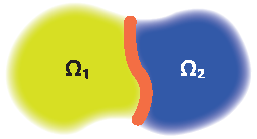
\includegraphics[width=5cm]{chapters/chapter3/figures/blob.pdf}
    \end{minipage}
    \begin{minipage}{0.45\textwidth}
        \begin{align*}
        E(\rOmega_{1}\cup\rOmega_2) &= E(\rOmega_1) + E(\rOmega_2) + W_{12} \qquad \\
        & \overset{?}{=}\mathcal{E}(\rOmega_1)+\mathcal{E}(\rOmega_2)
        \end{align*}
    \end{minipage}
\caption{
	The energy of an isolated system is the sum of the energies of its subsystems (as defined when they are isolated as well) plus the interaction among them, $W_{12}$, whose magnitude scales as the area of the interface, depicted in red. When defining the energies of individual subsystems, $\mathcal{E}$, $W_{12}$ has to be arbitrarily partitioned among them.
	}
	\label{fig:energy-partition}
\end{figure}

Let us consider a mono-atomic fluid interacting through pair potentials, $v(|\mathbf{R}_n-\mathbf{R}_m|)$, and define the atomic energies as \cite{Marcolongo2014,Ercole2016}:
\begin{equation}
  e_{\smallgamma,n}(\rGamma) =
  \frac{1}{2M_n}(\mathbf{P}_{n})^{2} + \frac{1}{2}\sum_{m\ne n}
  v(|\mathbf{R}_{n}-\mathbf{R}_{m}|)
  (1+\gamma_{nm}), \label{eq:gamma-atomic-energies}
\end{equation}
where $\gamma_{nm}=-\gamma_{mn}$ is \emph{any} antisymmetric matrix.
As the inter-atomic potential appearing in Eq.~\eqref{eq:gamma-atomic-energies} is symmetric with respect to the atomic indices, it is clear that the sum of all the atomic energies does not depend on $\gamma$, thus making any choice of $\gamma$ equally permissible. This trivial observation has deep consequences on the theory of thermal fluctuations and transport, because the value of the macroscopic energy flux, instead, depends explicitly on $\gamma$, thus making one fear that the resulting transport coefficients would depend on $\gamma$ as well. Using the same manipulations that lead from Eqs.~\eqref{eq:epsilon-classical} and \eqref{eq:atomic-energies} to Eq.~\eqref{eq:J-classical}, for any choice of the $\gamma$ matrix in Eq.~\eqref{eq:gamma-atomic-energies}, a corresponding expression for the macroscopic energy flux can be found, reading \cite{Marcolongo2014,Ercole2016}:
\begin{equation}
  \mathbf{J}_{\smallgamma}^\smallE=\mathbf{J}^\smallE+
  \frac{1}{2 \rOmega}\sum_{n,m\ne n}\gamma_{nm} \Bigl ( v_{nm} \mathbf{V}_{n} + \bigl (\mathbf{V}_{n}\cdot \nabla_{\mathbf{R}_n} v_{nm} \bigr )  (\mathbf{R}_{n}-\mathbf{R}_{m}) \Bigr ), \label{eq:gamma-classical-current}
\end{equation}
where $v_{nm}= v(|\mathbf{R}_{n} - \mathbf{R}_{m}|)$.

\begin{figure}
    \begin{center}
        \subfigure[\label{fig:argon-gauge-acf}]{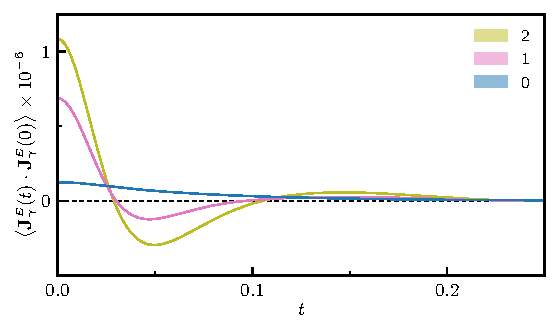
\includegraphics[width=0.8\textwidth]{chapters/chapter3/figures/handbook_argon_egauge_acf.pdf}}
        \subfigure[\label{fig:argon-gauge-kappa}]{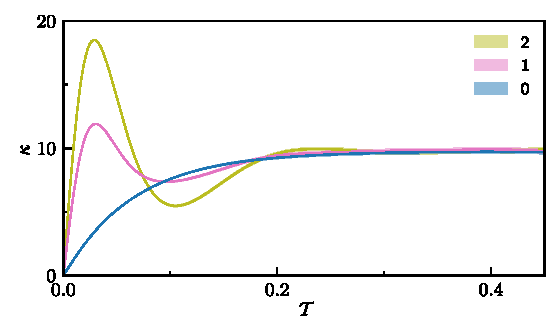
\includegraphics[width=0.8\textwidth]{chapters/chapter3/figures/handbook_argon_egauge_kappa.pdf}}
    \end{center}
	\caption{(a) Time correlation functions of the modified macroscopic energy flux of a Lennard-Jones fluid, at the conditions described in the text, as defined in Eq.~\eqref{eq:gamma-classical-current}, for different definitions of the $\gamma$ matrix (see text). The ``0'' line refers to the standard definition ($\gamma = 0$), whereas the labels ``1'' and ``2'' correspond to the two (arbitrary) definitions of $\gamma$ given in Eq.~\eqref{eq:gamma-definitions}.
    (b) Integral of the time correlation functions displayed in Fig.~\ref{fig:argon-gauge-acf}, multiplied by the prefactor appearing in the GK relation, Eq.~\eqref{eq:GK-complete}, as a function of the upper limit of integration. 
    The parameters used are $\lambda_1=10$ and $\lambda_2=2.5$. The barely visible shaded area surrounding each line is an indication of the error bars, as estimated by standard block analysis. Units are Lennard-Jones units ($M=\sigma=\varepsilon=1$). Reproduced from Ref.~\cite{Ercole2016}. 
    }
    \label{fig:argon-gauge}
\end{figure}

\subsection{An example from classical MD}
In order to illustrate this state of affairs, we have performed classical MD simulations for a Lennard-Jones monoatomic fluid described by the inter-atomic potential $v(R) = 4\varepsilon \left[ \left( \frac{\sigma}{R}\right)^{12} - \left(\frac{\sigma}{R} \right)^{6} \right]$ at temperature $T=1.86 \frac{\epsilon}{k_B}$ and density $\rho=0.925 \sigma^{-3}$, using cubic simulation cells containing 256 atoms in the iso-choric microcanonical ensemble, with the LAMMPS package \cite{LAMMPS1995}. 
We computed different definitions of the energy flux of Eq.~\eqref{eq:gamma-classical-current}, by choosing $\gamma$ matrices constructed in two different ways, according to the (arbitrary) prescriptions:
\begin{equation}
\setbox0=\vbox{\hsize=68mm \small\noindent where the matrix
      elements of $A$ are drawn from a uniform deviate  in the
      $[0,\lambda]$ interval.}
\setbox1 \vbox{\hsize=68mm \small\noindent according to whether $I=J$,
  $I>J$, or $I<J$.}
\gamma_{IJ}= \left \{
  \begin{alignedat}{2}
    \frac{1}{2} \left(A_{IJ}-A_{JI}\right ) & \quad\raise -0.3\ht0
    \box0 && \qquad (1) \\
\\
    0, +\lambda, -\lambda & \quad \box1 && \qquad (2) \\
  \end{alignedat} \right .
\label{eq:gamma-definitions}
\end{equation}
In Fig.~\ref{fig:argon-gauge-acf} we display the resulting macroscopic energy-flux autocorrelation functions, $\langle \mathbf{J}_{\gamma}^{\smallE}(t) \cdot \mathbf{J}_{\gamma}^{\smallE}(0) \rangle$, that dramatically depend on the definition of the $\gamma$ matrix in Eqs.~\eqref{eq:gamma-atomic-energies} and \eqref{eq:gamma-classical-current}.  Notwithstanding, the integrals of all these time correlation functions tend to the same limit at large integration times, as shown in Fig.~\ref{fig:argon-gauge-kappa}.

\begin{LEtext}
The ill-definetess of the atomic energies and of the heat current was already noticed by some authors. \citet{Schelling2002} computed the thermal conductivity of Stillinger-Weber \cite{Stillinger1985} silicon and noticed that it was fairly insensitive to the particular definition used, and concluded that the fact that there is no rigorous and unique definition is not a serious impediment to using the GK method. Ten years later, \citet{Howell2012} studied the same system more extensively, and found that the energy decomposition in the three-body interaction term gives a negligible contribution to the computed thermal conductivity, even though he did not recognize the ill-definiteness of the two-body atomic energy term.

How is it that different definitions of the energy flux would lead to the same value for the thermal conductivity? The fundamental origin of this conundrum involves two intrinsic properties of the total energy: \emph{extensivity} and \emph{conservation}, that lead us to the discovery of a gauge invariance principle for thermal transport coefficients.
\end{LEtext}


%%%%%%%%%%%%%%%%%%%%%%%%%%%%%%%%%%%%%%5
\section{Gauge invariance}  \label{sec:gauge-invariance}

In order to get insight into this remarkable invariance property, let us inspect the difference between the generalized flux in Eq.~\eqref{eq:gamma-classical-current} and the standard expression of Eq.~\eqref{eq:J-classical}:
\begin{equation}
  \rDelta\mathbf{J}^\smallE_{\smallgamma} =\mathbf{J}^\smallE_{\smallgamma}-\mathbf{J}^\smallE  =\frac{\mathrm{d}}{\mathrm{dt}}\frac{1}{4 \rOmega} \sum_{n,m\ne n}  \gamma_{nm} \, v(|\mathbf{R}_{n}-\mathbf{R}_{m}|)  (\mathbf{R}_{n}-\mathbf{R}_{m}). \label{eq:DeltaJ}
\end{equation}
We see that the two different expressions for the macroscopic energy flux differ by a total time derivative of a bounded phase-space vector function. In the following, we show that this is a consequence of energy conservation and extensivity and a sufficient condition for the corresponding thermal conductivities to coincide.

The very possibility of defining an energy current density, from which the energy fluxes of Eq.~\eqref{eq:J-classical} and \eqref{eq:gamma-classical-current} ultimately depend, stems from energy extensivity, \emph{i.e.} the energy of a macroscopic sample of matter of volume $\Omega$ can be written as the integral of an energy density, $e(\mathbf{r})$:
\begin{equation}
  E[\Omega]=\int_{\Omega}e(\mathbf{r})d\mathbf{r}. \label{eq:E-extensivity}
\end{equation}
Along the same considerations illustrated in Fig.~\ref{fig:energy-partition}, the energy density appearing in Eq. \eqref{eq:E-extensivity} is not uniquely defined:  any 
two densities $e'(\mathbf{r},t)$ and $e(\mathbf{r},t)$, whose integrals over a macroscopic volume differ by a quantity that scales as the volume boundary, should be considered as equivalent. 
This equivalence can be expressed by the condition that two equivalent densities differ by the divergence of a (bounded) vector field:
\begin{equation}
  e'(\mathbf{r},t)=e(\mathbf{r},t) - \nabla\cdot \bm{p}(\mathbf{r},t). \label{eq:gauge_transformation}
\end{equation}
In a sense, two equivalent energy densities can be thought of as different \emph{gauges} of the same scalar field. 

Energy is also conserved: because of this, for any given gauge of the energy density, $e(\mathbf{r},t)$, an energy current density can be defined, $\bm{j}(\mathbf{r},t)$, so as to satisfy the continuity equation, Eq.~\eqref{eq:continuity}:
\begin{equation}
  \dot{e}(\mathbf{r},t)=-\nabla\cdot
  \mathbf{j}_{e}(\mathbf{r},t). \label{eq:energy-continuity} 
\end{equation}
By combining Eqs.~\eqref{eq:gauge_transformation} and \eqref{eq:energy-continuity} we see that energy current densities and macroscopic fluxes transform under a gauge transformation as:
\begin{align}
 \bm{j}'(\mathbf{r},t) & = \bm{j}(\mathbf{r},t) + \dot{\bm{p}}(\mathbf{r},t), \label{eq:current_density_gauge} \\
  \mathbf{J}'(t) & = \mathbf{J}(t) + \dot{\mathbf{P}}(t), \label{eq:macroscopic_flux_gauge}
\end{align}
where $\mathbf{P}(t)=\frac{1}{\rOmega} \int\bm{p}(\mathbf{r},t)d\mathbf{r}$. We
conclude that the macroscopic energy fluxes in two different energy gauges differ by the total time derivative of a bounded phase-space vector function.

We now show that the energy fluxes of the same system in two different energy gauges, $e$ and $e'$, differing by a bounded total time derivative, as in Eq.~\eqref{eq:macroscopic_flux_gauge}, result in the same heat conductivity, as given by the Green-Kubo formula, Eq.~\eqref{eq:GK-complete}. More generally, the Onsager coefficients coupling two fluxes, $\mathbf{J}^1$ and $\left(\mathbf{J}^1\right)'$, do not depend on the gauge of either one of them. In fact, let $\left(\mathbf{J}^1\right)' = \mathbf{J}^1 + \dot{\mathbf{P}}$; one has:
\begin{equation}
  \begin{aligned}
    \left (L^{11} \right)' &= \frac{\rOmega}{2 k_B }\int_{-\infty}^{+\infty} \left \langle \left (\mathbf{J}^1(t)+\dot{\mathbf{P}}(t) \right ) \cdot  \left (\mathbf{J}^1(0)+\dot{\mathbf{P}}(0)\right ) \right \rangle dt \\
    &= L^{11} + \frac{\rOmega}{2 k_B } \left[ \left .  \left \langle \mathbf{P}(t) \cdot \dot{\mathbf{P}}(0) \right \rangle \right |^{+\infty}_{-\infty} + \left .  2 \Bigl \langle \mathbf{P}(t) \cdot \mathbf{J}^1(0) \Bigr \rangle \right |^{+\infty}_{-\infty} \right] ,
  \end{aligned} \label{eq:L=L'}
\end{equation}
where we used the property that classical auto-correlation functions are even in time.
The expectation of the time-lagged products in Eq.~\eqref{eq:L=L'} factorizes into the products of two independent expectations at large time lag. As the equilibrium expectations of both a total time derivative and a current vanish, we conclude that $\left (L^{11}\right )'=L^{11}$. Heat conductivities computed in different energy gauges coincide, as they must on physical grounds. A slight generalization of this argument, also using microscopic reversibility as in Ref.~\cite{Onsager1931a,Onsager1931b}, allows us to conclude that $\left (L^{12} \right )'=L^{12}$ and that, in general, $\kappa'=\kappa$.

We summarize the gauge invariance principle with a theorem.
\begin{theorem}[Gauge invariance] \label{th:gauge-invariance}
Two energy fluxes that differ by a total time derivative of a bounded function, result in the same thermal conductivity (Onsager coefficient).
\end{theorem}


\subsection{Alternative proof}
\begin{LEtext}
An alternative proof of the gauge invariance principle of the Onsager coefficients can be obtained using the Lemma described by \citet{Marcolongo2016}.

\begin{lemma}[\citeauthor{Marcolongo2016}] \label{th:aris-theorem}
Let $\mathbf{J}^A$ and $\mathbf{J}^B$ be two macroscopic fluxes defined for the same system, and  $\mathbf{J}^{C} = \mathbf{J}^A + \mathbf{J}^B$ be their sum. The corresponding Onsager coefficients\footnote{For the sake of simplicity, with $L^X$ we indicate the $(\smallone,\smallone)$ component of the Onsager matrix, built using $J^X$.
%but it is straightforward to generalize the theorem to the other components.
}, $L^{A}$, $L^{B}$, and $L^{C}$ satisfy the relation:
\begin{equation} \label{eq:aris-theorem}
    \left| L^{C} - L^{A} - L^{B} \right| \leq 2 \sqrt{L^{A} L^{B}}
\end{equation}
\end{lemma}

\begin{proof}
The Einstein-Helfand relation (Eq.~\eqref{eq:Einstein-Helfand-Lij}) correspondent to a flux $\mathbf{J}^X$ states that 
\begin{equation}
    L^{X} = \lim_{\mathcal{T}\rightarrow\infty} \frac{\left\langle|\mathbfcal{D}^X(\mathcal{T})|^2\right\rangle} {\mathcal{T}},
\end{equation}
where $\mathbfcal{D}^X(\mathcal{T})=\int_0^{\mathcal{T}} \mathbf{J}^X(t) dt$ is the displacement associated with the flux $\mathbf{J}^X$. It follows that:
\begin{equation}
    L^{C} = L^{A} + L^{B} + \lim_{\mathcal{T}\rightarrow\infty} \frac{2\left\langle \mathbfcal{D}^A(\mathcal{T}) \cdot \mathbfcal{D}^B(\mathcal{T})\right\rangle}{\textbf{}}.
\end{equation}
Canonical averages of products of phase-space functions can be seen as scalar products:\footnote{Let us consider two random variables, $X$ and $Y$, and $Z=(X+aY)^2$, where $a\in \mathbb{R}$ is a constant. By definition $Z$ is not negative, and $0\leq \langle Z \rangle = \langle X^2 \rangle + a^2 \langle Y^2 \rangle + 2a \langle XY \rangle$. If we take $a = -\frac{\langle XY \rangle}{\langle Y^2 \rangle}$, we obtain the Schwartz inequality
\begin{equation} \label{eq:schwartz-ineq}
    |\langle XY \rangle| \leq \sqrt{\langle X^2 \rangle} \sqrt{\langle Y^2 \rangle}.
\end{equation}}
therefore, thanks to the Cauchy-Schwartz inequality, we have that $\lim_{\mathcal{T}\rightarrow\infty} \frac{2\left\langle \mathbfcal{D}^A(\mathcal{T}) \cdot \mathbfcal{D}^B(\mathcal{T})\right\rangle}{\mathcal{T}} \leq 2\sqrt{L^{A} L^{B}}$, that proves the theorem. 
\end{proof}

\begin{proof}[Proof (alternative)]
Alternatively, we can express the Onsager coefficients as the zero-frequency value of the correspondent power spectrum (or cross spectrum), as in Eq.~\eqref{eq:GK-S0}, \emph{i.e.} $L^{X} \propto S^{XX}(\omega=0)$. We obtain:
\begin{align}
    S^{CC}(\omega=0) &= \int_{-\infty}^\infty \langle J^C(t) J^C(0) \rangle dt \nonumber\\
        &=\int_{-\infty}^\infty \left(\langle J^A(t) J^A(0) \rangle + \langle J^B(t) J^B(0) \rangle + 2\langle J^A(t) J^B(0) \rangle \right) dt  \nonumber\\
        &= S^{AA}(\omega=0) + S^{BB}(\omega=0) + 2 S^{AB}(\omega=0), \label{eq:aris-theorem-Scc}
\end{align}
where we used the fact the $\langle J^A(t) J^B(0) \rangle = \langle J^B(t) J^A(0) \rangle$, and from Eqs.~\eqref{eq:Sij(omega)} we have:
\begin{equation}
    S^{AB}(\omega=0) = \left\langle \frac{\int_0^\mathcal{T} J^A(t) dt}{\sqrt{\mathcal{T}}} \frac{\int_0^\mathcal{T} J^B(t) dt}{\sqrt{\mathcal{T}}} \right\rangle + \mathcal{O}(\mathcal{T}^{-1}) .
\end{equation}
Thanks to the Schwartz inequality (Eq.~\eqref{eq:schwartz-ineq}), we must have that
\begin{equation}
\begin{aligned}
    0 \leq \left|S^{AB}(\omega=0)\right| &\leq \sqrt{\left\langle\frac{1}{\mathcal{T}}\left(\int_0^\mathcal{T} J^A(t) dt\right)^2\right\rangle} \sqrt{\left\langle\frac{1}{\mathcal{T}}\left(\int_0^\mathcal{T} J^B(t) dt\right)^2\right\rangle} \\
    &\quad = \sqrt{S^{AA}(\omega=0) S^{BB}(\omega=0)} ,
\end{aligned} \label{eq:aris-theorem-Sab}
\end{equation}
for any $\mathcal{T}>0$. By letting $\mathcal{T}\rightarrow\infty$, Eq.~\eqref{eq:aris-theorem} follows from Eq.~\eqref{eq:aris-theorem-Scc} and \eqref{eq:aris-theorem-Sab}.
\end{proof}

\smallskip
Thanks this theorem, if we define $\mathbf{J}'(t)$ as in Eq.~\eqref{eq:macroscopic_flux_gauge}, we shall have that $\left| \kappa' - \kappa - \kappa_{\dot{\mathbf{P}}} \right| \leq 2 \sqrt{\kappa \kappa_{\dot{\mathbf{P}}}}$. Since $\mathbf{\dot{P}}$ is a bounded function and using the Einstein-Helfan relation (Eq.~\ref{eq:Einstein-Helfand-Lij}), we have that $\kappa_{\dot{\mathbf{P}}} = \lim_{\mathcal{T}\rightarrow\infty} \frac{\left\langle |\dot{\mathbf{P}}| \right\rangle}{\mathcal{T}} = 0$, hence $\kappa = \kappa'$. 
\end{LEtext}


\section{Molecular fluids}  \label{sec:MolecularFluids}
In a one-component molecular fluid such as liquid water or, say, ethanol, there are in general $Q$ fluxes interacting with each other through Onsagers' Eq.~\eqref{eq:onsager}, where $Q$ is the number of atomic species in a molecule. The requirement that atoms are bound in molecules of fixed composition, however, sets a number of constraints that substantially simplify the treatment of heat transport, making the molecular case similar to the one-component one.

Let us consider a molecule of chemical formula $A_{N_A} B_{N_B}\cdots$, where $A, B,\cdots$ indicate atomic species, and $N_A,N_B,\cdots$ the corresponding atomic stoichiometric indices. For each atomic species we define the normalized number flux as:
\begin{equation}
  \mathbf{J}^X = \frac{1}{N_X}\sum_{n\in X} \mathbf{V}_n. \label{eq:JX}
\end{equation}
If we indicate by $M_X$ the atomic mass of species $X$, momentum conservation requires that $\sum_X M_X N_X \mathbf{J}^X = 0$ in the center-of-mass reference frame. The flux $\mathbf{J}^{XY} = \mathbf{J}^{X}-\mathbf{J}^{Y}$ is the total time derivative of a bounded vector, because its integral is the sum over all the molecules of the difference between the average atomic positions of either species within a same molecule, which is obviously bounded if molecules do not dissociate. As any number flux $\mathbf{J}^X$ can be expressed as a linear combination of the total momentum and of several $\mathbf{J}^{XY}$ fluxes, each of them is the total time derivative of a bounded vector. Therefore, by the gauge invariance theorem, the Onsager coefficient coupling any of these atomic fluxes with any other or with the energy flux vanishes. We conclude that energy is the only conserved quantity relevant for heat transport in a molecular fluid, and that the energy-flux autocorrelation function directly yields the thermal conductivity, as in Eq.~\eqref{eq:GK}.


\section{Formation and self-energy contributions in heat currents}  \label{sec:gauge-renormalization}
\LEnote{*** Spiegazione dei metodi di scorrelazione / rinormalizzazione di Aris, per rimuovere i contributi delle self-energie. (se riesco... non se ha senso parlare anche dei metodi multi-componente ***}
\LEnote{** Ma forse questa sezione va spostata nel cap.5 (data analysis) ?***}


\section{Comment on the classical definition of heat flux in solids}  \label{sec:carbogno}
\LEnote{*** dimostrazione semplice con teorema di Aris che corrente ``Leyla'' = corrente di calore, e non vale per quella ``di Carbogno'' *** SE HO TEMPO, SPOSTO IN APPENDICE (o elimino)***}



\section{Outlook}  \label{sec:gauge-outlook}
\begin{LEtext}
The discovery of the gauge invariance principle provides the theoretical foundation for the formulation of a microscopic theory of adiabatic heat transport in the framework of density functional theory (DFT). The first such formulation is presented in Chapter~\ref{ch:dft-heat}. 

Furthermore, this principle opens the possibility of designing the definition of the local energy (both in terms of atomic energies or energy densities), so as to optimize the convergence of the thermal conductivity estimator.
The Marcolongo-Schwartz theorem, Eq.~\eqref{eq:aris-theorem}, ensures that if a flux $\mathbf{J}^B$ does not contribute to the conductivity (\emph{i.e.} it has a vanishing GK integral, $L^B=0$), it is possible to the define a new flux $\mathbf{J}^C=\mathbf{J}^A+\mathbf{J}^B$ that will yield the same conductivity of $\mathbf{J}^A$. Even though $L^C=L^A$, the statistical properties of two such equivalent currents need not be the same, in that the fluctuations of their correlation functions will be different, and the resulting GK integral, Eq.~\eqref{eq:GK-complete} will depend differently on the upper limit of integration, as it was the case in the example shown in Fig.~\ref{fig:argon-gauge}.
We shall see that in the particular case of DFT thermal transport, for some peculiar systems, the natural definition of energy density and flux may make the estimate of the thermal conductivity very difficult, due to the large statistical fluctuations of the correlation functions. In this cases, the gauge invariance principle can come to the rescue.

Besides, the general concept of gauge invariance of heat conductivity will likely apply to other transport properties as well, such as ionic conduction, viscosity, and many others, and/or simulation methodologies, such as those based on a neural-network representation of interatomic potentials, which hold the promise of a strong and long-lasting impact on molecular simulations. 
\end{LEtext}
\LEnote{**CIT. Martin per gauge invariance viscosity?**}
